\documentclass[a4paper,10pt,twocolumn,oneside]{article}
\usepackage[bottom=1in,top=0.5in,left=0.5in,right=0.5in]{geometry}
\usepackage{upquote}
\usepackage{listings}
\usepackage{dejavu}
\usepackage{graphicx}
\usepackage{hyperref}
\usepackage{mathtools}
\lstset{
    language=C++,
    basicstyle=\footnotesize\ttfamily,
    breaklines=true,
    breakatwhitespace=true,
    tabsize=2,
    morekeywords={constexpr},
}
\title{JAW Codebook}
\author{}
\date{}

\begin{document}
\maketitle
\tableofcontents

\section{Basic}
\subsection{vimrc}
\lstinputlisting{../codes/0000-vimrc}

\section{Data Structure}
\subsection{Undo Disjoint Set}
\lstinputlisting{../codes/1010-undo-disjoint-set.cpp}
\subsection{Range Disjoint Set}
\lstinputlisting{../codes/1020-range-disjoint-set.cpp}

\subsection{Treap}
\lstinputlisting{../codes/treap_pointer.cpp}
\subsection {Heavy Light Decomposition}
\lstinputlisting{../codes/main_one_SegTree.cpp}
\subsection {Link Cut Tree}
\lstinputlisting{../codes/1050-link-cut-tree.cpp}

\section{Graph}
\subsection{BCC Edge}
\lstinputlisting{../codes/bcc_edge.cpp}
\subsection{BCC Vertex}
\lstinputlisting{../codes/bcc_vertex.cpp}
\subsection{Strongly Connected Components}
\lstinputlisting{../codes/kosaraju.cpp}
\subsection{DMST\_with\_sol}
\lstinputlisting{../codes/dmst_sol.cpp}
\subsection{Dominator Tree}
\lstinputlisting{../codes/DominatorTree.cpp}
\subsection{Maximum Clique}
\lstinputlisting{../codes/2060-bron-kerbosch.cpp}
\subsection{MinimumMeanCycle}
\lstinputlisting{../codes/MinMeanCycle.cpp}

\section{Flow}
\subsection{Push-relabel} %Checked
\lstinputlisting{../codes/push-relabel.cpp}
\subsection{Dinic} %Checked
\lstinputlisting{../codes/dinic.cpp}
\subsection{Cost Flow} %Checked
\lstinputlisting{../codes/CostFlow.cpp}
\subsection{Kuhn Munkres}
\lstinputlisting{../codes/3040-kuhn-munkres.cpp}
\subsection{SW-Mincut}
\lstinputlisting{../codes/SW-mincut.cpp}
\subsection{Maximum Matching}
\lstinputlisting{../codes/3060-maximum-matching.cpp}
\subsection{Minimum Weight Matching (Clique version)}
\lstinputlisting{../codes/Minimum_General_Weighted_Matching.cpp}
\subsection{(+1) SW-mincut $O(NM)$}
\lstinputlisting{../codes/p1SWcutNM.cpp}

\section{Math}
\subsection{Linear Inverse Table}
\lstinputlisting{../codes/4005-linear-inverse-table.cpp}
\subsection{ax+by=gcd}
\lstinputlisting{../codes/ax+by=gcd.cpp}
\subsection{Fast Fourier Transform}
\lstinputlisting{../codes/4020-fast-fourier-transform.cpp}
\subsection{Fast Linear Recurrence}
\lstinputlisting{../codes/4030-fast-linear-recurrence.cpp}
\subsection{(+1) ntt}
\lstinputlisting{../codes/p1_ntt.cpp}
\subsection{Mod}
\lstinputlisting{../codes/MOD.cpp}
\subsection{Miller Rabin}
\lstinputlisting{../codes/4060-miller-rabin.cpp}
\subsection{Pollard Rho}
\lstinputlisting{../codes/4070-pollard-rho.cpp}
\subsection{Algorithms about Primes}
$12721$,
$13331$,
$14341$,
$75577$,
$123457$,
$222557$,
$556679$,
$999983$,
$98789101$,
$100102021$,
$987654361$,
$987777733$,
$999888733$,
$999991231$,
$999991921$,
$999997771$,
$1000512343$,
$1001010013$,
$1010101333$,
$1010102101$,
$1076767633$,
$1097774749$,
$1000000000039$,
$1000000000000037$,
$2305843009213693951$,
$4611686018427387847$,
$9223372036854775783$,
$18446744073709551557$
\lstinputlisting{../codes/primes.cpp}
\subsection{Count Coprime Pairs}
\lstinputlisting{../codes/4085-count-coprime-pairs.cpp}
\subsection{(+1) PolynomialGenerator}
\lstinputlisting{../codes/PolyGen.cpp}
\subsection{Pseudoinverse of Square matrix}
\lstinputlisting{../codes/Square_Matrix_pinv.cpp}
\subsection{Simplex}
\lstinputlisting{../codes/Simplex.cpp}

\subsection{Lucas's Theorem}
For non-negative integers $n$, $m$ and a prime $p$,
\[{m\choose n} \equiv \prod_{i=0}^{k}{m_i\choose n_i} \pmod{p},\]
where $m_i$ and $n_i$ are base $p$ expansions of $m$ and $n$, respectively.
\subsection{Pick's Theorem}
Given a simple polygon of which all vertices are lattice points
with area $A$, $i$ interior lattice points, and $b$ boundary lattice points,
we have \[A=i+{b\over2}-1.\]
\subsection{Kirchhoff's Theorem}
Given a simple graph $G$ with $n$ vertices.
Let \[L_{i,j} \coloneqq
\begin{dcases}
    deg(v_i) & \text{if } i = j \\
    -1 & \text{if } i \ne j \text{ and } v_i \text{ is adjacent to } v_j \\
    0 & \text{otherwise}
\end{dcases}.
\]
Then for any $i$ and $j$,
\# of spanning trees of $G$ is \[\det \widehat{L_{i,j}}.\]
\section{Geometry}
\subsection{Point operators}
\lstinputlisting{../codes/pdd.cpp}
\subsection{Intersection of two circles}
\lstinputlisting{../codes/Intersection_of_two_circles.cpp}
\subsection{Intersection of two lines}
\lstinputlisting{../codes/Intersection_of_two_lines.cpp}
% XXX wrong when intersection is empty
\subsection{Half Plane Intersection}
\lstinputlisting{../codes/5040-half-plane-intersection.cpp}
\subsection{2D Convex Hull}
\lstinputlisting{../codes/convex_hull.cpp}
\subsection{3D Convex Hull}
\lstinputlisting{../codes/3D_convex_hull.cpp}
\subsection{Minimum Covering Circle}
\lstinputlisting{../codes/mcc.cpp}
\subsection{KDTree (Nearest Point)}
\lstinputlisting{../codes/KD_Tree.cpp}
\subsection{Triangulation}
\lstinputlisting{../codes/triangulation.cpp}

\section{Stringology}
\subsection{Suffix Array}
\lstinputlisting{../codes/6010-suffix-array.cpp}
\subsection{Suffix Array (SAIS TWT514)}
\lstinputlisting{../codes/sais_twt514.cpp}
\subsection{Aho-Corasick Algorithm}
\lstinputlisting{../codes/Aho-Corasick.cpp}
\subsection{KMP}
\lstinputlisting{../codes/kmp.cpp}
\subsection{Z value}
\lstinputlisting{../codes/zvalue.cpp}
\subsection{Z value (palindrome ver.)}
\lstinputlisting{../codes/zvalue_palindrome.cpp}
\subsection{Palindromic Tree}
\lstinputlisting{../codes/6070-palindromic-tree.cpp}
\subsection{Lexicographically Smallest Rotation}
\lstinputlisting{../codes/smallest_rotation.cpp}
\subsection{Suffix Automaton}
\lstinputlisting{../codes/6090-suffix-automaton.cpp}

\section{Problems}
\subsection{Mo's Algorithm on Tree}
\lstinputlisting{../codes/7010-mos-algorithm-on-tree.cpp}
\subsection{Manhattan MST}
\lstinputlisting{../codes/ManhattanMST.cpp}

\clearpage
\section{Miscellany}
\subsection{tabi no hidarite saihate no migite}
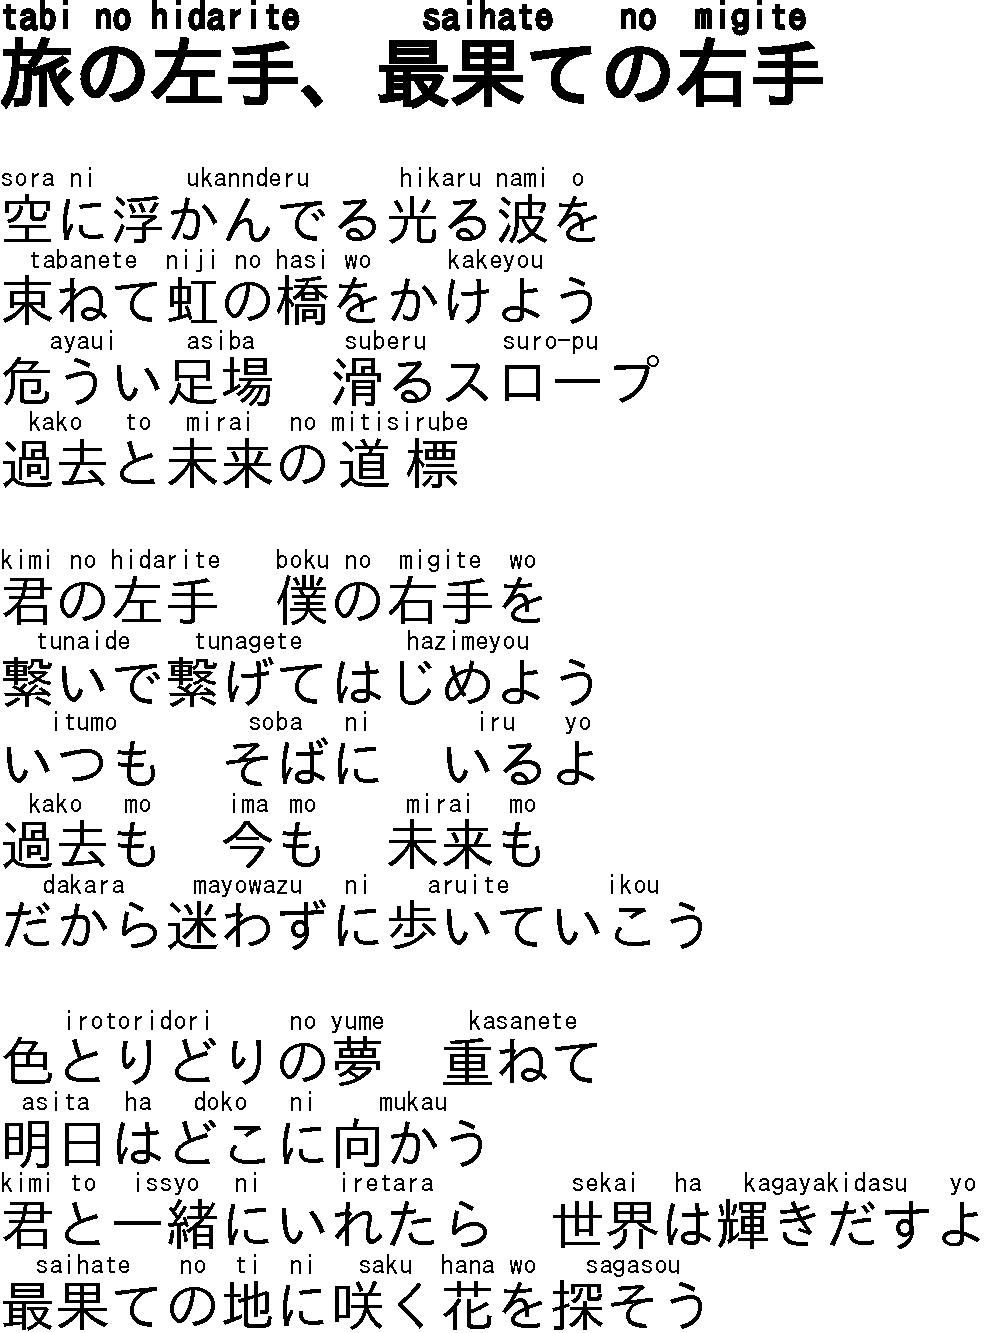
\includegraphics{../images/tabinohidaritesaihatenomigite}
\clearpage
\subsection{Made in Abyss}
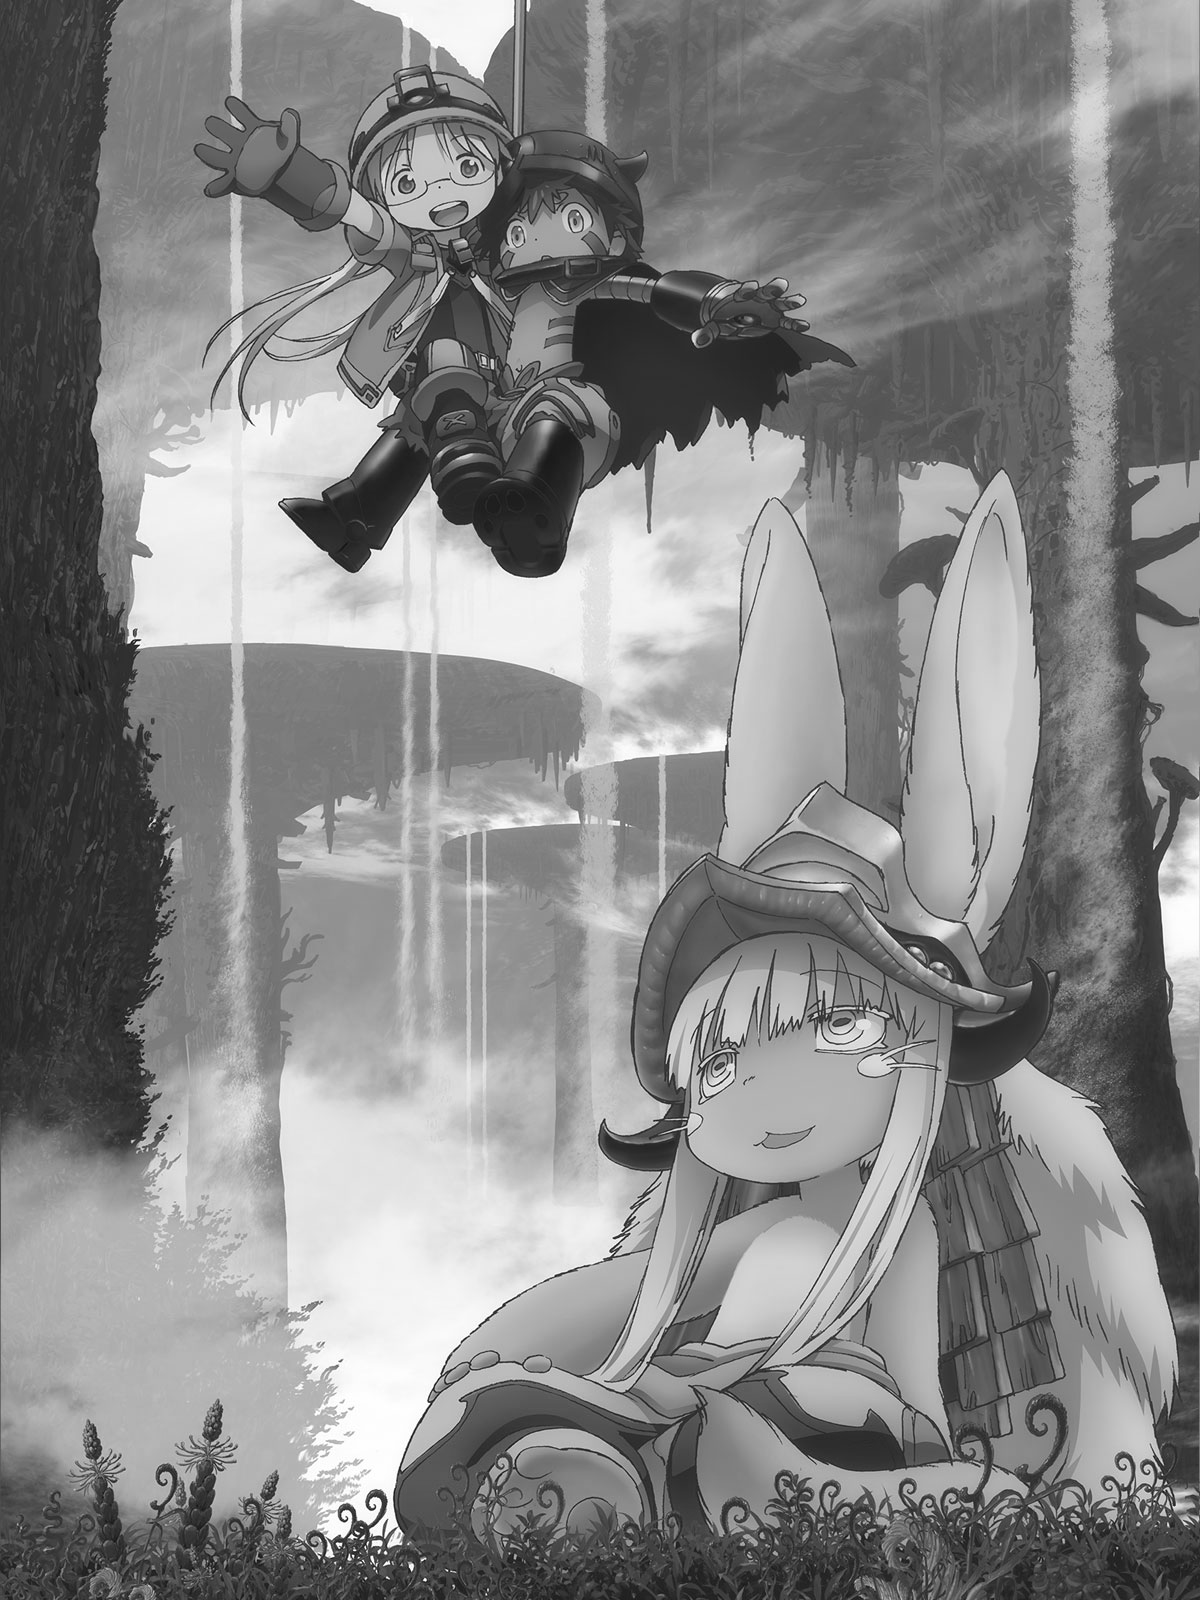
\includegraphics[width=7in]{../images/miabyss}
\end{document}
